\documentclass[a4paper, 10pt]{article}
\usepackage[english]{babel}
\usepackage[utf8]{inputenc}
\usepackage{amsfonts}
\usepackage{graphicx}
\usepackage[hidelinks]{hyperref}

\author{Maarten de Jonge}
\title{Projective Geometric Algebra}

\begin{document}
\newcommand{\rp}{$\mathbb{R}^{3,3}$}

\maketitle

\section*{Literature Review}
Li and Zhang\cite{hangbo2011} model line geometry in $\mathbb{R}^{3,3}$,
representing lines as vectors that square to zero (\emph{null vectors}). This
generalises the Pl\"{u}cker coordinate representation of lines to a proper
geometric algebra. The 6D vector of a line's Pl\"{u}cker coordinates corresponds
to the coordinates of of the line's direction and moment on a basis of 2-blades
in $\wedge^2(V^4)$, a bivector space over a 4D homogeneous vector space. The
also provide a metric for this space, turning it into $\mathbb{R}^{3, 3}$.
They proceed to give geometrics interpretations of the various blades that can
be formed in $\mathbb{R}^{3, 3}$.

Pottmann and Wallner\cite{pottmann2001computational} do similarly, except using
linear algebra rather than geometric algebra as Li and Zhang did.

Leo Dorst\cite{dorst2013versors} provides visualisations for many of the
geometric features described by \cite{hangbo2011} and
\cite{pottmann2001computational} and describes how to extract the parameters
required for implementing these visualisations.
GAViewer\footnote{\url{http://www.geometricalgebra.net/gaviewer\_download.html}},
a visualisation tool/graphical calculator for geometric algebra which handles
many different models of the algebra. Patrick de Kok\cite{dekok2012} implemented
the Pl\"{u}cker model of \cite{hangbo2011} in GAViewer and added many of the
visualisations described by \cite{dorst2013versors}.

\section*{Research Question}
At the time of \cite{dekok2012}, not all blades of \rp were able to be
visualised. A recent breakthrough by Dorst allows for the visualisation of
3-blades formed by three skew lines, which form a \emph{regulus} (figure
\ref{fig:regulus}). I will continue Patrick's work and implement this missing
visualisation.

\begin{figure}[htbp]
  \centering
  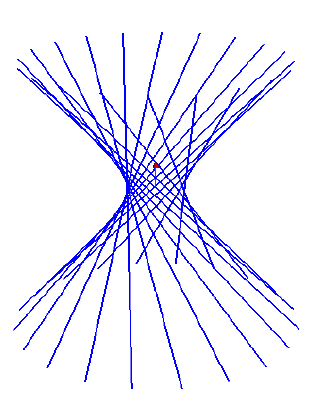
\includegraphics[width=0.5\textwidth]{regulus.png}
  \caption{A regulus}
  \label{fig:regulus}
\end{figure}

Also, something else.

%The further direction of the project is still up for consideration. One of the
%options is to apply projective geometric algebra to 2D projective geometry in
%the same vein as the Cinderella
%software\footnote{\url{http://doc.cinderella.de/tiki-index.php?page=Theoretical+Background}},
%and compare the results (in terms of e.g. performance, ease of implementation,
%elegance, or other such metrics) of the geometric algebra approach with the
%complex linear algebra used by Cinderella.

\section{Method and Approach}
The project can be roughly divided into 3 parts:
\begin{itemize}
  \item Becoming familiar with the field of projective line geometry and the
    required algebra\"{i}c knowledge.
  \item Implementing the GAViewer visualisations.
  \item The other thing.
\end{itemize}

\bibliographystyle{plain}
\bibliography{library}
\end{document}
